%%%%%%%%%%%%%%%%%%%%%%%%%%%%%%%%%%%%%%%%%%%%%%%%%%%%%%%%%%%%%%%%%%%%%%%%%%%%%%%%
\documentclass[11pt]{article} % Dokumentenklasse

\usepackage[utf8]{inputenc} % Textkodierung: UTF-8
\usepackage[T1]{fontenc} % Zeichensatzkodierung

\usepackage[USenglish]{babel}% http://ctan.org/pkg/babel
\usepackage{graphicx} % Grafiken
\usepackage[absolute]{textpos} % Positionierung

% Schriftart Helvetica:
\usepackage[scaled]{helvet}
\renewcommand{\familydefault}{\sfdefault}

\usepackage{calc} % Berechnungen
\usepackage{tabto} % Tabulatoren
\usepackage{parskip}

\usepackage{enumitem}

% Debugging:
%\usepackage{layout} % Layout-Informationen
%\usepackage{printlen} % Längenwerte ausgeben

%%%%%%%%%%%%%%%%%%%%%%%%%%%%%%%%%%%%%%%%%%%%%%%%%%%%%%%%%%%%%%%%%%%%%%%%%%%%%%%%
% EINSTELLUNGEN
%%%%%%%%%%%%%%%%%%%%%%%%%%%%%%%%%%%%%%%%%%%%%%%%%%%%%%%%%%%%%%%%%%%%%%%%%%%%%%%%

% Seitenränder:
\newcommand{\SeitenrandOben}{43.5mm}
\newcommand{\SeitenrandRechts}{20mm}
\newcommand{\SeitenrandLinks}{20mm}
\newcommand{\SeitenrandUnten}{10mm}

\newcommand{\UniversitaetLogoBreite}{19mm}
\newcommand{\UniversitaetLogoHoehe}{1cm}

\usepackage[a4paper,
top=\SeitenrandOben,
bottom=\SeitenrandUnten,
inner=\SeitenrandLinks,
outer=\SeitenrandRechts,
foot=0cm,
head=0cm
]{geometry}

\textblockorigin{\SeitenrandLinks}{\SeitenrandOben} % Ursprung für Positionierung

\setlength{\parindent}{0pt}
%\setlength{\baselineskip}{32pt}
\setlength{\parskip}{\baselineskip}
\TabPositions{4cm}
\pagestyle{empty}

%%%%%%%%%%%%%%%%%%%%%%%%%%%%%%%%%%%%%%%%%%%%%%%%%%%%%%%%%%%%%%%%%%%%%%%%%%%%%%%%
% General stuff
%%%%%%%%%%%%%%%%%%%%%%%%%%%%%%%%%%%%%%%%%%%%%%%%%%%%%%%%%%%%%%%%%%%%%%%%%%%%%%%%
\newcommand{\Problem}[1]{\paragraph*{Problem #1:}\qquad}
\newcommand{\Topic}[1]{
	\newpage
	\section*{#1}}

\newcommand{\Given}{\textbf{Given:\qquad\qquad}}
\newcommand{\Searched}{\textbf{Searched:\qquad}}
\newcommand{\Solution}{\textbf{Solution:\qquad}}

%%%%%%%%%%%%%%%%%%%%%%%%%%%%%%%%%%%%%%%%%%%%%%%%%%%%%%%%%%%%%%%%%%%%%%%%%%%%%%%%
% Math stuff
%%%%%%%%%%%%%%%%%%%%%%%%%%%%%%%%%%%%%%%%%%%%%%%%%%%%%%%%%%%%%%%%%%%%%%%%%%%%%%%%
\usepackage{amsmath}
\usepackage{amssymb}

\newcommand{\R}{\mathbb{R}}
\newcommand{\Vector}[1]{\R^{#1}}
\newcommand{\Matrix}[2]{\R^{#1 \times #2}} % !!! DON'T TOUCH !!!
%%%%%%%%%%%%%%%%%%%%%%%%%%%%%%%%%%%%%%%%%%%%%%%%%%%%%%%%%%%%%%%%%%%%%%%%%%%%%%%%


\newcommand{\ExerciseNumber}{10}

\newcommand{\PersonOne}{Marcel Bruckner (03674122)}
\newcommand{\PersonTwo}{Julian Hohenadel (03673879)}
\newcommand{\PersonThree}{Kevin Bein (03707775)}


%%%%%%%%%%%%%%%%%%%%%%%%%%%%%%%%%%%%%%%%%%%%%%%%%%%%%%%%%%%%%%%%%%%%%%%%%%%%%%%%
% DOKUMENT
%%%%%%%%%%%%%%%%%%%%%%%%%%%%%%%%%%%%%%%%%%%%%%%%%%%%%%%%%%%%%%%%%%%%%%%%%%%%%%%%

\begin{document}

%%%%%%%%%%%%%%%%%%%%%%%%%%%%%%%%%%%%%%%%%%%%%%%%%%%%%%%%%%%%%%%%%%%%%%%%%%%%%%%%
\begin{textblock*}{\UniversitaetLogoBreite}[1,0](\textwidth-1mm, 2cm-\SeitenrandOben)%
	\raggedleft
\includegraphics{../Ressources/Universitaet_Logo_RGB.pdf}%
\end{textblock*}


\begin{textblock*}{\textwidth}[0,0](0cm, 0cm)%
	{\fontsize{24pt}{26pt}\selectfont\textbf{Exercise}}
	
	\vspace*{14pt}
	{\fontsize{18pt}{27pt}\selectfont\textbf{\ExerciseNumber}}
\end{textblock*}

\vspace*{92.2mm}
\fontsize{15pt}{17.5pt}\selectfont%
TUM Department of Informatics

\renewcommand{\baselinestretch}{1.47}
\normalsize\selectfont
\vspace*{17.1mm}
\textbf{Supervised by}\tab
\begin{minipage}[t]{\textwidth-\CurrentLineWidth}
	Prof. Dr. Stephan Günnemann\\
	Informatics 3 - Professorship of Data Mining and Analytics\strut
\end{minipage}

\vspace*{4.3mm}
\textbf{Submitted by}\tab
\begin{minipage}[t]{\textwidth-\CurrentLineWidth}
	\PersonOne\\
	\PersonTwo\\
	\PersonThree
\end{minipage}

\vspace*{-1mm}
\textbf{Submission date}\tab 
\begin{minipage}[t]{\textwidth-\CurrentLineWidth}
	Munich, \today
\end{minipage}
\newpage % !!! DON'T TOUCH !!!
%%%%%%%%%%%%%%%%%%%%%%%%%%%%%%%%%%%%%%%%%%%%%%%%%%%%%%%%%%%%%%%%%%%%%%%%%%%%%%%%

%%%%%%%%%%%%%%%%%%%%%%%%%%%%%%%%%%%%%%%%%%%%%%%%%%%%%%%%%%%%%%%%%%%%%%%%%%%%%%%%
% !!! HOMEWORK STARTS HERE !!!
%%%%%%%%%%%%%%%%%%%%%%%%%%%%%%%%%%%%%%%%%%%%%%%%%%%%%%%%%%%%%%%%%%%%%%%%%%%%%%%%
%
\Topic{Deep Learning II}
%
\Problem{1}
%
\begin{flushleft}
a) Since all weights are positive, $\max(0, W_j^{*^T} x_i) = W_j^{*^T}x_i$ and the following holds:
\begin{align*}
	\mathcal{L}_{NN}(W^*_{NN}) &= \frac{1}{2} \sum_{i=1}^N ( - y_i)^2 \\
	&= \frac{1}{2} \sum_{i=1}^N (  W_{L+1}^{*^T} (W_L^{*^T} \max(0, \ldots(0, W_2^{*^T}\max(0, W_1^{*^T} x_i)))) - y_i)^2 \\
	&= \frac{1}{2} \sum_{i=1}^N (  W_{L+1}^{*^T} (W_L^{*^T}(\ldots ( W_2^{*^T}( W_1^{*^T} x_i)))) - y_i)^2 \\
	&= \frac{1}{2} \sum_{i=1}^N (  W_{L+1}^{*^T} \cdot \ldots \cdot  W_1^{*^T} x_i - y_i)^2 \\
	&= \frac{1}{2} \sum_{i=1}^N (  W_{NN}^{*^T} x_i - y_i)^2 
\end{align*}
Since the solutions $W^*_{NN}$ and $w^*_{LS}$ are a global optimum, we can set $W_{NN}^* = w_{LS}^*$ and we get $\mathcal{L}_{NN}(W^*_{NN}) = \mathcal{L}_{LS}(w^*_{LS})$.
\end{flushleft}

\begin{flushleft}
b) Since simple linear regression is a special case of a Feed-Forward Neural Network, the Loss is the same. This does not work the other way around because NNs can learn more complex functions. $w^*_{LS}$ being non-negative does not imply anything about the optimal weights of the network $W^*_{NN}$.Therefore we can conclude that  $\mathcal{L}_{NN}(W^*_{NN}) \leq \mathcal{L}_{LS}(w^*_{LS})$.
\end{flushleft}
%
%
\Problem{2}
%
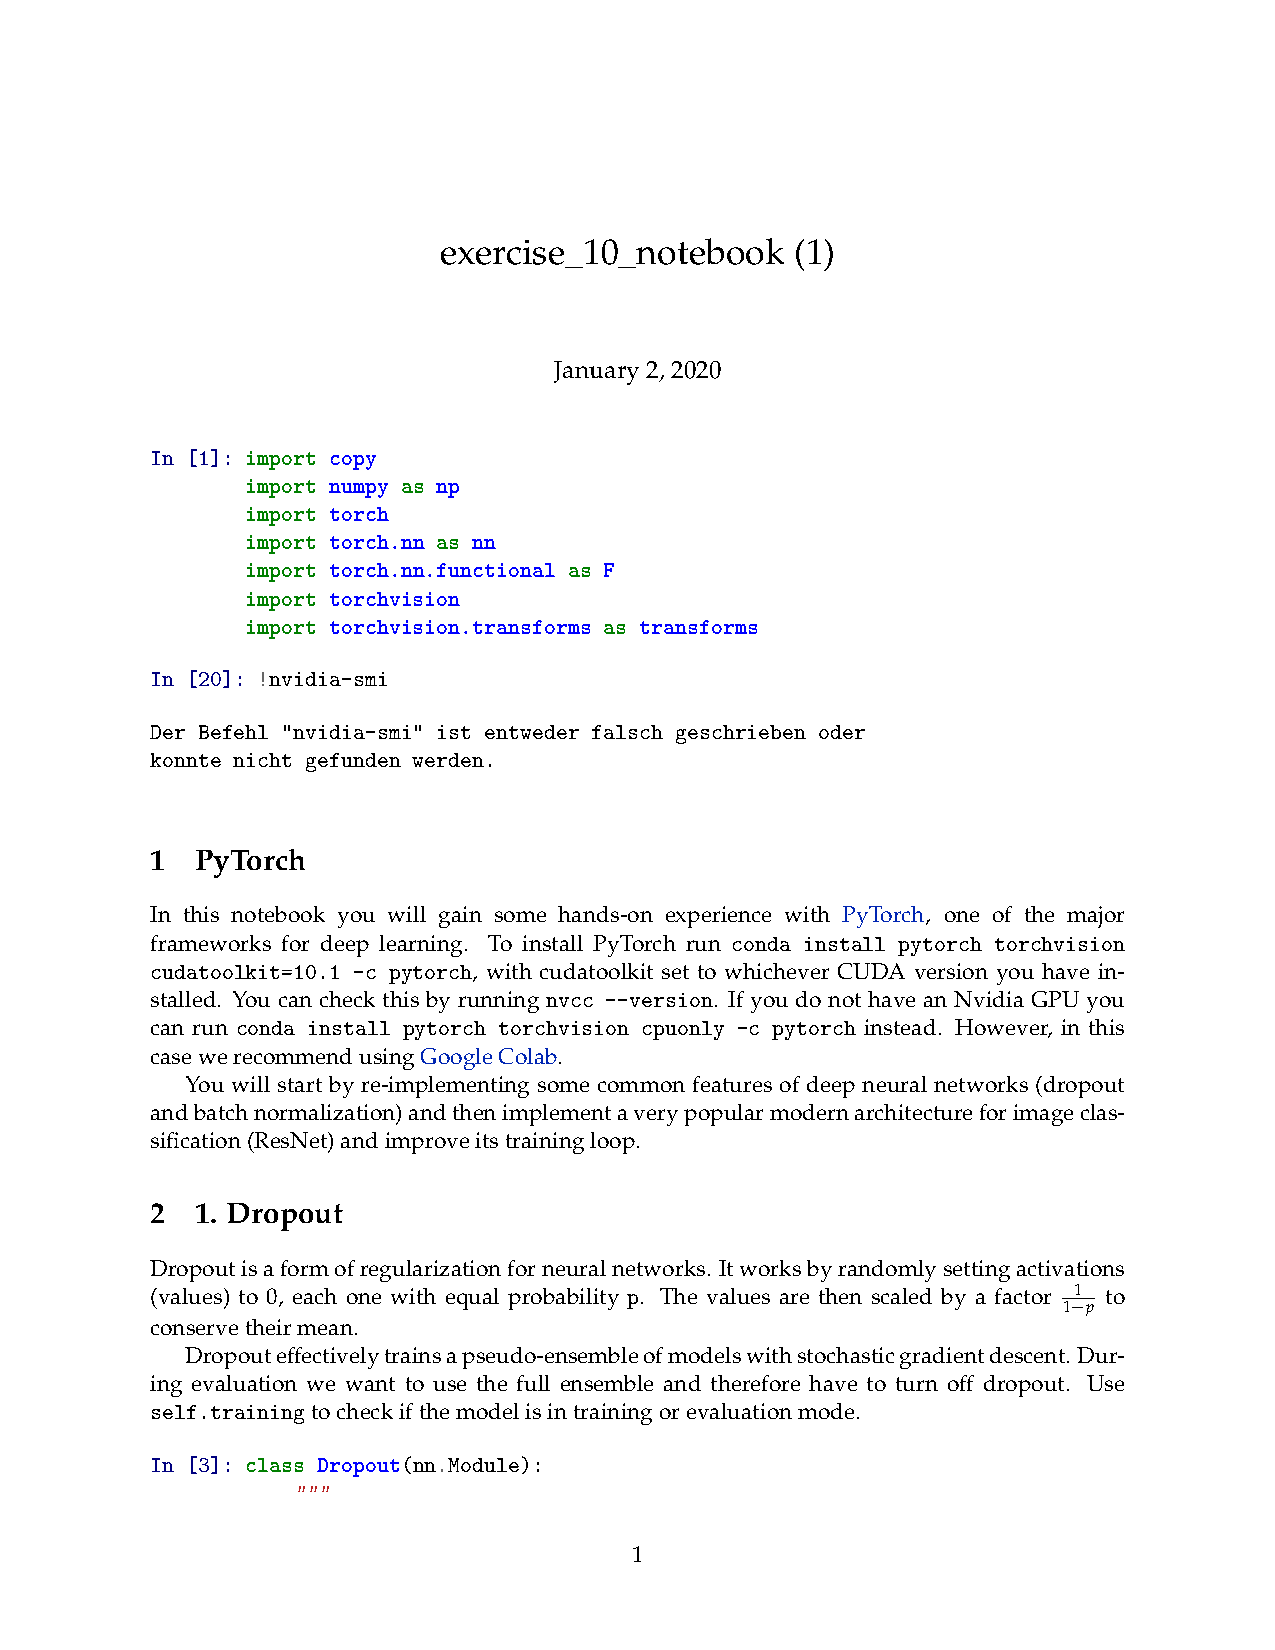
\includepdf[pages=-]{exercise_10_notebook.pdf}
%
%

%%%%%%%%%%%%%%%%%%%%%%%%%%%%%%%%%%%%%%%%%%%%%%%%%%%%%%%%%%%%%%%%%%%%%%%%%%%%%%%%
% !!! HOMEWORK ENDS HERE !!!
%%%%%%%%%%%%%%%%%%%%%%%%%%%%%%%%%%%%%%%%%%%%%%%%%%%%%%%%%%%%%%%%%%%%%%%%%%%%%%%%

%%%%%%%%%%%%%%%%%%%%%%%%%%%%%%%%%%%%%%%%%%%%%%%%%%%%%%%%%%%%%%%%%%%%%%%%%%%%%%%%
\newpage

\vspace*{-15.8mm}
\fontsize{19pt}{21pt}\selectfont

\vspace{25.3mm}
Appendix

\normalsize\selectfont
\vspace{13.2mm}
We confirm that the submitted solution is original work and was written by us without further assistance. Appropriate credit has been given where reference has been made to the work of others.

\vspace{18.1mm}
\rule[-3.7mm]{\linewidth}{0.5pt}
Munich, \today, Signature \PersonOne

\vspace{18.1mm}
\rule[-3.7mm]{\linewidth}{0.5pt}
Munich, \today, Signature \PersonTwo

\vspace{18.1mm}
\rule[-3.7mm]{\linewidth}{0.5pt}
Munich, \today, Signature \PersonThree
 % !!! DON'T TOUCH !!!
%%%%%%%%%%%%%%%%%%%%%%%%%%%%%%%%%%%%%%%%%%%%%%%%%%%%%%%%%%%%%%%%%%%%%%%%%%%%%%%%

\end{document}
